\documentclass[border=4pt]{standalone}
\usepackage[T1]{fontenc}
\usepackage{helvet}
\renewcommand{\familydefault}{\sfdefault}
\usepackage{graphicx}
\usepackage{caption}
\usepackage{amsmath}
\captionsetup{font={sf,footnotesize},labelfont={sf,bf,footnotesize},justification=justified,singlelinecheck=false}
\begin{document}
\setcounter{figure}{5}
\begin{minipage}{7.20in}
\centering
\begin{figure}[htbp]
    \centering
    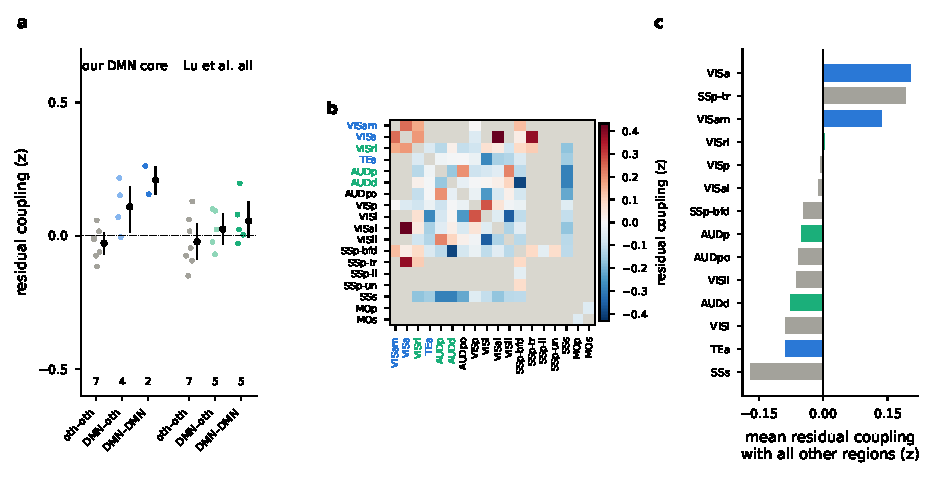
\includegraphics[width=\linewidth]{fig6_meso_panels.pdf}
    \caption{\textbf{a} Mesoscope grey-screen period: sessions with $\geq$200 s (most canonical sessions have only 60 s) and motion energy to verify stillness, 13 sessions, 7 mice (all 23 long sessions, without the motion-energy requirement, give the same ordering). Region-averaged calcium activity in still 1 s bins with nuisance regression; coupling as residual from the distance-matched mean; dots are mice, black mean and 95\% mouse-bootstrap CI; numbers at the bottom give the mice per class (DMN-DMN pairs come from 2 mice, mostly adjacent VISa-VISam). No frontal DMN region is imaged in these sessions; the wheel is logged in only 8 of the 23 long sessions. \textbf{b} Residual coupling of every imaged region pair present in $\geq$2 mice (grey: pair not imaged in $\geq$2 mice; regions without any such pair omitted), ordered posterior DMN, Lu temporal (TEa, AUD), visual, somatosensory, motor; tick colours as in Fig. 3. \textbf{c} Mean residual coupling of each region with all other imaged regions (pairs in $\geq$2 mice). VISa and VISam are the most coupled regions together with trunk somatosensory cortex (SSp-tr); RSP has too few pairs in this subset; the auditory areas and TEa (Lu et al. temporal module) are among the least coupled.}
    \label{fig:grey_meso}
\end{figure}
\end{minipage}
\end{document}
